\subsection{Modelado}


\subsection{Modelado Del Juego}

El juego en si consistirá en una lista de listas donde cada lista representará una columna del tablero. En cada turno un jugador elejirá una columna numerada del 0 al n, siendo n el numero de columnas totales y el juego se encargará. Ambos jugadores contarán en el momento de la elección con el estado actual del tablero.

Luego de cada jugada, el juego chequará si el jugador ganó o si ya no hay mas movimientos posibles, terminando el juego e informando que jugador gano o si fue empate.

El pseudocodigo del juego será, entonces el siguiente:

\begin{algorithm}[h!]
\begin{algorithmic}[1]\parskip=1mm
 \caption{jugar()}
 \STATE{While True}
 \STATE{\quad columna = player.move(tablero)}
 \STATE{\quad jugar\_ficha(columna, tablero)}
 \STATE{\quad if jugador\_gano(tablero)}
 \STATE{\quad\quad return player}
 \STATE{\quad if tablero\_lleno(tablero)}
 \STATE{\quad\quad return empate}
 \STATE{\quad player = otro\_jugador(player)}
\end{algorithmic}
\end{algorithm}

Como ya adelantamos en la introducción, es necesario definir en que etapa del algoritmo se le asignará la recompensa al algoritmo de q-learning. Una opción bastante sencilla e intuitiva es la de asignar recompensas en el momento en que algun jugador gana la partida. Por ejemplo al ganar la partida uno de los jugadores, se le asigna una recompensa de $1$ a el y una recompensa de $-1$ al contrincante. Siguiendo con el lineamiento anterior, tambien sería posible asignarles recompensas en el momento en que se empata, por ejemplo, asignandoles a ambos jugadores una recompensa de $0.5$

En caso de que no se haya llegado a un estado final, una posible propuesta es asignarle al otro jugador una recompenza por ejemplo de 0.

El pseudocodigo entonces, pasaría a verse de la siguiente manera:

\begin{algorithm}[h!]
\begin{algorithmic}[1]\parskip=1mm
 \caption{jugar()}
 \STATE{While True}
 \STATE{\quad columna = player.move(tablero)}
 \STATE{\quad jugar\_ficha(columna, tablero)}
 \STATE{\quad if jugador\_gano(tablero)}
 \STATE{\quad\quad player.recompensa(1)}
 \STATE{\quad\quad otro\_jugador(player).recompensa(-1)}
 \STATE{\quad\quad return player}
 \STATE{\quad if tablero\_lleno(tablero)}
 \STATE{\quad\quad player.recompensa(0.5)}
 \STATE{\quad\quad otro\_jugador(player).recompensa(0.5)}
 \STATE{\quad\quad return empate}
 \STATE{\quad otro\_jugador(player).recompensa(0)}
 \STATE{\quad player = otro\_jugador(player)}
\end{algorithmic}
\end{algorithm}


\subsection{Modelado De Jugadores}

Un jugador estará compuesto por dos metodos basicos, uno que llamaremos $move()$ que, dado un estado del tablero devuleve una acción valida (tirar ficha en la primera columna, en la segunda, etc) y una función $reward()$ que nos dirá en que estado quedo el juego luego de movernos y de que el oponente moviera y una recompensa que utilizaremos para actualizar la matriz $Q$ en caso de que el jugador lo requiera.

En particular, para la clase jugador que implemente q-learning el algoritmo para decidir que acción realizar vendrá dado de la siguiente manera:

\begin{algorithm}[h!]
\begin{algorithmic}[1]\parskip=1mm
 \caption{move(tablero)}
 \STATE{acciones\_validas = elegir\_acciones\_validas(tablero)}
 \STATE{Para cada acción en acciones\_validas}
 \STATE{\quad obtener q para accion}
 \STATE{\quad guardarlo en lista de qs\_validos}
 \STATE{accion\_elegida = elegir\_acción(acciones\_validas,qs\_validos)}
 \STATE{retornar accion\_elegida}
\end{algorithmic}
\end{algorithm}

Y la función learn, que basicamente consiste en adaptar la función de aprendisaje vista en la teorica:

\begin{algorithm}[h!]
\begin{algorithmic}[1]\parskip=1mm
 \caption{learn(tablero,recomensa)}
 \STATE{prev\_q = getQ(estado\_previo, accion\_elegida)}
 \STATE{maxqnew = tomar maximo q de tomar una acción en el tablero resultante}
 \STATE{q[(estado\_previo, accion\_elegida)] = prev + $\alpha$ * ((reward + $\gamma$*maxqnew) - prev)}
\end{algorithmic}
\end{algorithm}

Aqui quedan por definir varios parametros, entre ellos $\alpha$, $\gamma$ y los valores iniciales para la matriz $Q$. En primera instancia decidimos tomar valores que concideramos apropiados de a cuerdo a datos empiricos de la implementación y que concideramos razonables. Tomaremos $\alpha=0.4 $, $\gamma=0.9$ y todas los valores de Q iniciarán con $1$.

En la siguiente sección propondremos distintos algoritmos para elejir una acción tomado del jugador y teorizar como estas impactan en el aprendisaje.

\subsection{Planteo De Distintas Estrategias de Movimiento}

En esta sección plantearemos distintas estrategias que utilizará nuestro jugador al momento de elegir si explorar nuevas posibilidades o utilizar el mejor camino conocido.

En particular plantearemos estas tres estrategias:

%capaz no usar itemize?

\begin{itemize}
\item Estrategia Greedy: toma un camino random con probabilidad $\epsilon\%$ y en caso contrario utilice el mejor brazo conocido.
\item Estrategia $\epsilon$-first: toma un camino random en las primeras $\epsilon$ iteraciones y luego toma el mejor camino conocido.
\item Estrategia Softmax: basada en una función probabilistica que desarrollaremos a continuación.
\end{itemize}

La estrategia Softmax se basa en darle probabilidades distintas a cada acción posible dependiendo de la recomensa esperada de cada una de ellas.

En particular la probabilidad de cada una de las acciones vendrá dada por:

%imagen1.svg

 La variable $\tau$ se denomina parametro de temperatura, para temperaturas cercanas a infinito todas las acciones tienen aproximadamente la misma probabilidad de ser elegidas, mientras que para temperaturas bajas (cercanas a cero) la probabilidad de la accion de mayor recompensa tenderá a $1$.

En particular nuestra estrategia consistirá en comenzar con una temperatura alta para favorecer la exploración e ir gradualemente disminuyendola para favorecer mas a aquellas con mayor recopensa. Faltará definir de manera experimental cual será el valor inicial de $\tau$ y de que manera reduciremos su valor (algunas posiblidades son de manera linea, logaritmica, etc).


%Analisis De Exploración

\subsection{Analisis Espacio De Estados}

Segun el modelo planteado para la resolución del problema, la matriz Q tendrá como como columnas los diferentes estados en los que se puede encontrar el tablero y como filas las acciones que se pueden realizar sobre ese determinado tablero. Dado que la cantidad de estados diferentes en los que se puede encontrar el tablero tiene complegidad PSPACE y que la cantidad la acciones es acotada (a lo sumo m), podemos determinar que la complegidad espacial de nuestro algoritmo esta en PSPACE... not cool.

Si bien esto hace que la complegidad de explorar cada una de las posibilidades sea extremadamente costosa, consideramos que para la mayoría de los casos no es necesario concer todo el arbol sino los estados mas generales.

%referencia http://www.tzi.de/~edelkamp/publications/conf/ki/EdelkampK08-1.pdf


\pagebreak
\section{Experimentación}

\section{Estrategias vs Jugador Random}

Como primera instancia en la etapa de experimentación, haremos competir a un jugador q-learner contra un jugador que elige entre los posibles movimientos con probabilidad uniforme. Utilizaremos las tres estrategias enunciadas previamente para ver como se comporta cada una. 

La metodología utilizada para observar como evoluciona el algoritmo de q-learning será la de hacer jugar a ambos jugadores $10000$ veces randomizando cual es el que comienza primero. Luego tomaremos estos resultados y cada $200$ juegos, graficaremos cuantas veces ganó el algoritmo q-learning. 

Para la estrategia greedy, eligiendo un $\epsilon=0.1$ obtuvimos los siguientes resultados:

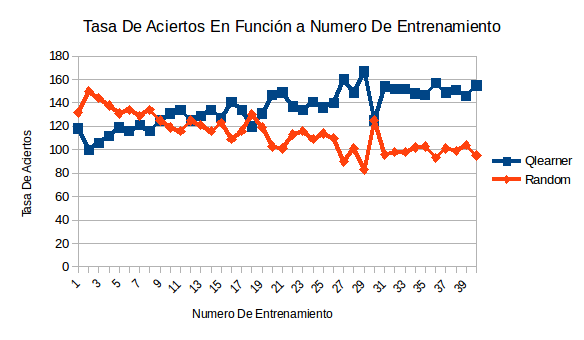
\includegraphics[scale=0.5]{testing/greedy.png}

%concluciones

Para la estrategia $\epsilon$-first eligiendo un $\epsilon=10\%$, y los resultados fueron los siguientes:

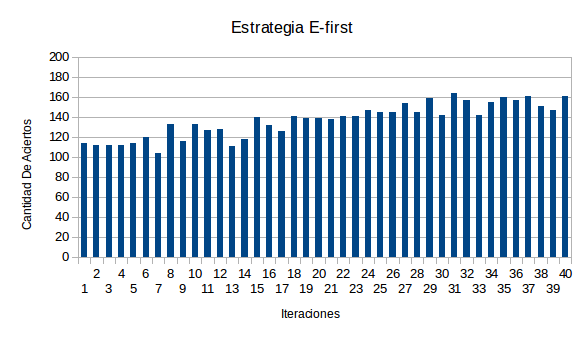
\includegraphics[scale=0.5]{testing/ef.png}

Puede verse como en el primer $10\%$ de las iteraciones el algorimo gana la mitad de las veces y prierde la otra mitad, lo que era de esperarse para una politica completamente random.

Con la tercera politica Soft-Max, decidimos utilizar una temperatura incial igual a $1$ y una función de calor que decrese de manera logaritmica con cada iteración:

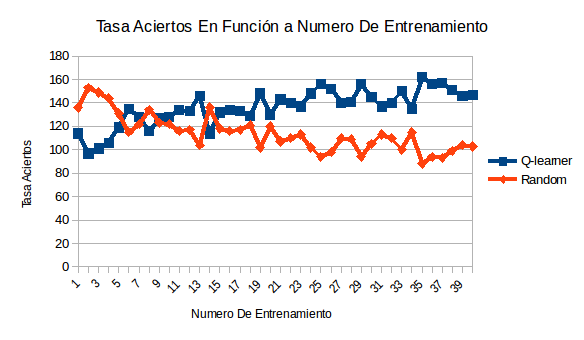
\includegraphics[scale=0.5]{testing/softmax.png}

%concluciones

\subsection{Performance de dos q-learners compitiendo}



\subsection{Performance al cambiar la inicialización de Q}
